	\chapter{Einf\"uhrung in Nvidia CUDA}
	Seit 2007 existiert das Nvidia Produkt \textit{Compute Unified Device Architecture} (CUDA). Dabei handelt es sich um eine Programmiersprache, eine Compilerarchitektur, eine Runtime-Library oder kurz gesagt um eine Plattform. CUDA lässt sich mit dem \textit{Nvidia CUDA Toolkit} leicht auf Linux, MacOS oder Windows installieren und bringt dabei mehrere HPC Bibliotheken mit. Auf einige soll später noch eingegangen werden. Die wichtigsten Vertreter sind:
	\begin{itemize}
		\item \textbf{cuBLAS}:   Die CUDA Implementierung der \textit{Basic Linear Algebra Subprograms}.
		\item \textbf{curand}:   Ein Zufallszahlen-Generator (RNG) und verschiedene Verteilungen.
		\item \textbf{cuSOLVER}: Eine Implementierung der beliebtesten Matrixzerlegungen.
		\item \textbf{THRUST}:   Die CUDA Implementierung der C++ Standard Template Library (STL).
	\end{itemize}
	Andere prominente Vertreter sind cuDNN, TensorRT und offizielle Partnerprojekte wie MAGMA, GROMACS oder Tensorflow.
				
		
		\section{C Runtime}
		Ein Hauptprogramm auf der CPU wird üblicherweise in C oder C++ geschrieben. Wahlweise lässt sich auch ein \Gls{API} in einer anderen Programmiersprache benutzen, z.B. pyCUDA in Python. Dieses Programm läuft wie gewohnt auf der CPU und wird fortan als Hostcode bezeichnet. Eine sehr rechenintensive Stelle im  Hostcode soll nun auf die GPU ausgelagert werden. Im gleichen Quellcode wird nun in der Programmiersprache CUDA ein sogenanntes \Gls{Kernel} definiert.
			\subsection*{Kernels}
			\Glspl{Kernel} sind sehr kleine Recheneinheiten, die parallel auf der GPU ausgeführt werden sollen. Der folgende Code zeigt ein \Gls{Kernel} zur Addition zweier Vektoren.
	  		\begin{lstlisting}[caption=Vektoraddition Kernel]
				__global__ void VecAdd(float* A, float* B, float* C, int N)
				{
    				int i = threadIdx.x;
    				if (i < N)
        				C[i] = A[i] + B[i];
				}
				
				...
				
				int main()
				{		
					...
					VecAdd<<<1, N>>>(A, B, C, N) ;
					...
				}
			\end{lstlisting}
			
			\Glspl{Kernel} werden immer mit dem Keyword \li`__global__` deklariert und der Rückgabetyp ist immer \li`void`. \Gls{Kernel}aufrufe erfolgen asynchron, d.h. die CPU schickt den Auftrag lediglich ab und arbeitet dann weiter den Hostcode ab. Mehrere \Gls{Kernel}aufrufe hintereinander werden auf der GPU serialisiert.
			
			Die spitzen Klammern geben an, mit welchen \Glspl{Thread} der Code ausgeführt werden soll. Im obigen Fall wird das \Gls{Kernel} mit $N$ \Glspl{Thread} gestartet. Ausnahmslos jeder dieser \Glspl{Thread} erhält das \Gls{Kernel} und führt den Code aus: Jeder \Gls{Thread} rechnet sich seinen Index aus (entspricht dem Prozessor-rank). Jeder \Gls{Thread} nimmt einen Wert von A und B, rechnet die Summe aus und schreibt genau einen Wert von C. Ein \Gls{Kernel} kann man sich also so vorstellen, als würde man eine Schleife ausrollen und jedes Element einzeln und parallel berechnen. \Glspl{Kernel} können nicht auf Hostcode zugreifen. Sollte $N$ größer sein als die Länge der Vektoren, so müssen die überzähligen \Glspl{Thread} warten. Ein Weglassen der if-Abfrage würde jedoch nicht zwingend zu einem Fehler führen. Um falsche Speicherzugriffe zu vermeiden, kann das Tool \li`cuda-memcheck` verwendet werden. (später mehr)
			
			Zur besseren Steuerung der \Glspl{Thread} teilt man diese in \Glspl{Block} ein\footnote{Meistens existieren technische Obergrenzen für die Zahl an Threads pro Block.}. Die Gesamtheit an \Glspl{Block}n bezeichnet man als \Gls{Grid}.
			
			\begin{lstlisting}[caption=Kernelaufruf]		
				int main()
				{
					int threadsPerBlock = 256;
					int blocksPerGrid = N / threadsPerBlock;
					
					...
					
					VecAdd<<<blocksPerGrid, threadsPerBlock>>>(A, B, C, N);
					
					...					
				}
			\end{lstlisting}

			In diesem Beispiel übergibt man im ersten Element zwischen den spitzen Klammern die Zahl an \Glspl{Block}n und im zweiten die Zahl an \Glspl{Thread} pro \Gls{Block}. Beide Zahlen multipliziert ergeben also die Zahl an \Glspl{Thread} insgesamt. Mittels \li`blockIdx.x*blockDim.x + threadIdx.x` berechnet man den globalen Index eines \Glspl{Thread}. Die \Glspl{MTIU} verteilen die \Glspl{Block} dann automatisch auf die \Gls{SM}. Sollten mehr \Glspl{Thread} involviert werden als tatsächlich zur Verfügung stehen, so wird zuerst eine passende Anzahl verteilt und dann für die restlichen \Glspl{Block} wiederholt. Der Index zählt dabei korrekt weiter, da er von der ID des \Gls{Block}s abhängt.
			
			Falls das \Gls{Kernel} eine Funktion aufrufen soll, so muss diese extra für das Device geschrieben werden. Dazu deklariert man diese Funktionen mit dem Keyword \li`__device__`. Analog dazu werden gewöhnliche Funktionen auf der CPU mit \li`__host__` deklariert. Wird kein Keyword geschrieben, so handelt es sich um eine Host Funktion. Wird eine Funktion mit beidem deklariert, so wird die Funktion für Device und Host kompiliert. Device Funktionen können nicht vom Host gerufen werden und umgekehrt. Eine Device Funktion darf einen return Wert haben.
			
			\subsection*{C++ Kompatibilit\"at}
			Die Programmiersprache CUDA orientiert sich an C11. Es können alle Features dieses Standards benutzt werden. C++ Code als Device Code zu schreiben ist allerdings wesentlich schwieriger und wurde daher nur teilweise implementiert. Eine Liste der C++ Features enthält der CUDA Programming Guide in Anhang F. \autocite{cudaPG} 
			
			
		\section{Speichermodell}
		Eine GPU kennt mindestens fünf Arten von Speicher:
		\begin{itemize}
			\item \Gls{global Memory}: Daten, die vom CPU Speicher kopiert werden, werden in diesem gespeichert. Dieser Speicher ist ausnahmslos allen \Glspl{Thread} zugänglich.
			\item \Gls{constant Memory}: Ein ebenfalls globaler Speicher. Konstante Variablen werden so read-only abgespeichert und verhalten sich ähnlich den konstanten Variablen in C (Vermeidung von Bankkonflikten).
			\item \Gls{local Memory}: Jeder \Gls{Thread} verfügt über einen sehr kleinen Speicher für Hilfsvariablen, die nur diesem zugänglich sind. Definiert man eine Variable im Devicecode, so wandert sie in den lokalen Speicher (z.B. der Index \li`int i`). Dieser Speicher ist ähnlich langsam wie \gls{global Memory}, wird aber in einen Cache geladen.
			\item \Gls{shared Memory}: Ein kleiner, extrem schneller Speicher, den sich jeweils die \Glspl{Thread} einer \Gls{SM} teilen. Pro \Gls{SM} ist ein Element in der GPU integriert.
			\item \Gls{texture Memory}: Ein interpolierender, globaler Speicher, der für Texturen, also multidimensionale Speicherstrukturen optimiert wurde.
		\end{itemize}
		
		\newpage
		
		\subsection{global Memory}
		Um die Vektoraddition von oben durchzuführen, muss die CPU zunächst die Vektoren in den \Gls{global Memory} kopieren. Folgendes Beispiel illustriert dies:		
		\begin{lstlisting}[caption=Vektoraddition Host]
			uint N = 256;
			uint size = N * sizeof(float);
			float ∗h_A = (float ∗)malloc(size);
			float ∗h_B = (float ∗)malloc(size);
			float ∗h_C = (float ∗)malloc(size);

			float ∗d_A;
			cudaMalloc(&d_A, size);
			float ∗d_B;
			cudaMalloc(&d_B, size);
			float ∗d_C;
			cudaMalloc(&d_C, size);
			
			
			cudaMemcpy(d_A, h_A, size, cudaMemcpyHostToDevice);
			cudaMemcpy(d_B, h_B, size, cudaMemcpyHostToDevice);

			int threadsPerBlock = 32;
			int blocksPerGrid = N / threadsPerBlock ;
			VecAdd<<<blocksPerGrid, threadsPerBlock>>>(d_A, d_B, d_C, N);
			cudaMemcpy(h_C, d_C, size, cudaMemcpyDeviceToHost);
			
			cudaFree(d_A); cudaFree(d_B); cudaFree(d_C);
			free(h_A); free(h_B); free(h_C);
		\end{lstlisting}	
		
		Der Befehl \li`cudaMalloc` erstellt einen Buffer der entsprechenden Größe im \Gls{global Memory}.
		Der Befehl \li`cudaMemcpy` kopiert dann den Speicher des Hostvektors in den Devicevektor auf der Grafikkarte. Dabei gibt \li`size` die Anzahl an Bytes an, die kopiert werden soll. Für eine einzelne Variable ($N$) ist dies nicht notwendig.
		Nachdem das Kernel abgeschickt wurde, wird der Ergebnisvektor auf den Host zurück kopiert. Auf die Pointervariablen lässt sich mittels Pointeraddition ein Offset angeben, die Größe muss aber entsprechend angepasst werden. Beispielhaft kopiert \li`(d_A+3, h_A+5, 20, ...)` exakt 20 Bytes beginnend von \li`h_A[5]` nach \li`d_A[3]`.
		Es ist zu beachten, dass \Gls{Kernel}aufrufe im Gegensatz zu den meisten \Gls{API}-Calls normalerweise asynchron laufen, also die CPU nicht blockieren (non-blocking). 
		Speicher auf dem Device wird mit \li`cudaFree` freigegeben.
		
		\subsection{shared Memory}
		\Gls{shared Memory} wird mit dem Keyword \li`__shared__` deklariert. Der erste \Gls{Thread}, der in einem \Gls{Kernel} auf eine solche Instruktion trifft, legt eine Variable im \gls{shared Memory} der entsprechenden Größe an. Diese Variable teilen sich dann alle \Glspl{Thread} eines \Gls{Block}s. Existieren insgesamt $n$ \Glspl{Block}, so existieren auch $n$ verschiedene Variablen. In der statischen Variante muss die Größe des Arrays zur Compile-Zeit bekannt sein.
		\begin{lstlisting}[caption=shared Memory statisch]
			__global__ void test()
			{
  				__shared__ int s[64];
  				...
			}
  		\end{lstlisting}

		Im Gegensatz zur statischen Variante lässt sich \gls{shared Memory} auch dynamisch allozieren:  		
  		\begin{lstlisting}[caption=shared Memory dynamisch]
			__global__ void test()
			{
  				extern __shared__ int s[];
  				...
			}
			
			int main()
			{
				...
				int shared_memory_size = ...
				test<<<1, threadsPerBlock, shared_memory_size>>>();
				...
			}			
  		\end{lstlisting}
  		
        Dem \Gls{Kernel} muss die Größe des \gls{shared Memory} (pro \Gls{Block}) mitgegeben werden. In beiden Fällen wird also das Allozieren des Speichers von der CPU übernommen.  Dynamische Speicherverwaltung ist mittlerweile auch auf dem Device möglich. Darauf wird jedoch erst später eingegangen (siehe Abschnitt \ref{sync}). 
        
        Sollen mehrere Arrays im \gls{shared Memory} abgelegt werden, so definiert man sich lediglich Pointer auf ein großes Gesamtarray. Der Beginn des jeweils neuen Arrays sollte sinnvollerweise dem Ende des vorangegangenen entsprechen.  	  		
  		\begin{lstlisting}	[caption=shared Memory verteilt]	
			extern __shared__ int s[];
			int *integerData = s;                        
			float *floatData = (float*)&integerData[nI];
			char *charData = (char*)&floatData[nF];
			
			...
			
			test<<<1, threadsPerBlock, 
				nI*sizeof(int) + nF*sizeof(float) + nC*sizeof(char)>>>(...);
		\end{lstlisting}

		Im folgenden Beispiel wird die Vektoraddition umgeschrieben, um sich die Vektoren A und B in den \gls{shared Memory} zu laden:	
		
		\begin{lstlisting}[caption=Vektoraddition shared Memory]
			__global__ void VecAdd(float* A, float* B, float* C, int N)
			{
    			int i = blockDim.x * blockIdx.x + threadIdx.x;
    			int tid = threadIdx.x;
    			
    			__shared__ float As[<blockDim.x>];
    			__shared__ float Bs[<blockDim.x>]; 			
    			if (i < N)
    			{
    			    As[tid] = A[i];
    			    Bs[tid] = B[i];  
    			    ...	    
        			C[i] = As[tid] + B[tid];
        		}
			}
		\end{lstlisting}
		
		Da ohnehin einmal \li`A[i]` und \li`B[i]` aus dem Speicher geladen werden müssen, ist es hier unsinnig, den Speicher überflüssigerweise zu kopieren. Allerdings könnten ja vor der Addition \li`As` und \li`Bs` noch mehrmals gebraucht werden. Die Aufgabe des Programmierers ist es nun herauszufinden, bei welcher Datengröße abhängig vom Algorithmus der \Gls{Performance}gewinn durch die höhere Bandbreite den Verlust durch das Kopieren übersteigt.
		
		\subsection{constant Memory}
		\Gls{constant Memory} wird mit dem Keyword \li`__constant__` als globale Variable deklariert. Mit dem Befehl \li`cudaMemcpyToSymbol` wird diese dann in den Speicher der GPU kopiert und steht dort dann auch global zur Verfügung, muss also beim \Gls{Kernel}aufruf nicht explizit angegeben werden:
		\begin{lstlisting}[caption=Vektoraddition constant Memory]
			__constant__ float d_A[12800];
			__global__ void VecAdd(float* B, float* C, int N)
			{
    			int i = blockDim.x * blockIdx.x + threadIdx.x;
    			if (i < N)
        			C[i] = d_A[i] + B[i];
			}
			
			...
			
			cudaMemcpyToSymbol(d_A, h_A, size);
			VecAdd<<<blocksPerGrid, threadsPerBlock>>>(d_B, d_C, N);
		\end{lstlisting}
		
		Der \gls{constant Memory} ist ebenfalls ein globaler Speicher und steht jedem \Gls{Thread} zur Verfügung. Allerdings müssen Aufrufe der selben Stelle im Speicher zur selben Zeit innerhalb eines \Glspl{Warp} (Bankkonflikt) nicht serialisiert werden. Daher eignet sich dieser Speicher besonders für konstante Skalare, z.B. Naturkonstanten.
		
		\subsection{Texture Memory}
		
		\subsection{Host Memory}
		
		\newpage
		\section{Mehrdimensionale Bl\"ocke}
		Bisher wurden \Gls{Kernel} immer nur mit eindimensionalen \Glspl{Block}n und \Glspl{Grid} ausgeführt. Allerdings verbirgt sich dahinter ein Typecast. Zum Beispiel wird \li`<<<1,N>>>` zu \li`<<<dim3(1,1,1), dim3(N,1,1)>>>`. \li`dim3` bezeichnet dabei eine eingebaute Datenstruktur, die aus drei vorzeichenlosen Ganzzahlen besteht. In diesem Fall gibt sie die Anzahl der \Glspl{Block} im \Gls{Grid} bzw. der \Glspl{Thread} pro \Gls{Block} in die Raumrichtungen \li`(x,y,z)` an. Das \Gls{Grid} und die \Glspl{Block} sind also keine Ketten sondern Quader von Objekten. Die Indizes der \Glspl{Block} und \Glspl{Thread} lassen sich dann Spalten-, Zeilen- und Ebenen-weise abfragen: 			
		\begin{lstlisting}[caption=Multidimensionale Blöcke]
			__global__ test()
			{
				int row = blockIdx.y * blockDim.y + threadIdx.y;
				int col = blockIdx.x * blockDim.x + threadIdx.x;
				...
			}
    		
    		...

		    dim3 dimBlock(BLOCK_SIZE, BLOCK_SIZE);
    		dim3 dimGrid(GRID_SIZE, GRID_SIZE;
    		test<<<dimGrid, dimBlock>>>();
		\end{lstlisting}
        In diesem Fall werden also \Glspl{Block} der Größe \li`BLOCK_SIZE`$\times$\li`BLOCK_SIZE` in einem \Gls{Grid} mit \li`GRID_SIZE`$\times$\li`GRID_SIZE` \Glspl{Block}n angeordnet. Bei modernen GPUs ist die Obergrenze für die Dimension der \Glspl{Block} \li`(1024,1024,64)`.
        
        Das folgende Beispiel behandelt die Matrixmultiplikation unter Zuhilfenahme von \gls{shared Memory} und Multidimensionalen \Glspl{Block}n:       
        \begin{lstlisting}[caption=Matrixmultiplikation]
			#define BLOCK_SIZE 16 	
			typedef struct
			{
				uint width;
				uint height;
				float* elements;
				uint stride;
			} Matrix;

			__device__ 
			float GetElement(const Matrix A, uint row, uint col)
			{
				return A.elements[row * A.stride + col];
			}

			__device__ 
			void SetElement(Matrix A, uint row, uint col, float value)
			{
				A.elements[row * A.stride + col] = value;
			}
			
			__device__
			Matrix GetSubMatrix(Matrix A, uint row, uint col) 
			{
				Matrix Asub;
				Asub.width    = BLOCK_SIZE;
				Asub.height   = BLOCK_SIZE;
				Asub.stride   = A.stride;
				Asub.elements = &A.elements[A.stride * BLOCK_SIZE * row 
					+ BLOCK_SIZE * col];
				return Asub;
			}	
			 
			__global__ 
			void MatMulKernelShared(const Matrix A, const Matrix B, Matrix C)
			{    
    			uint blockRow = blockIdx.y;
    			uint blockCol = blockIdx.x;

    			Matrix Csub = GetSubMatrix(C, blockRow, blockCol);
    
    			float Cvalue = 0;

    			uint row = threadIdx.y;
    			uint col = threadIdx.x;

    			for (uint m = 0; m < (A.width / BLOCK_SIZE); ++m)
    			{
					Matrix Asub = GetSubMatrix(A, blockRow, m);
					Matrix Bsub = GetSubMatrix(B, m, blockCol);

					__shared__ float As[BLOCK_SIZE][BLOCK_SIZE];
					__shared__ float Bs[BLOCK_SIZE][BLOCK_SIZE];
					As[row][col] = GetElement(Asub, row, col);
					Bs[row][col] = GetElement(Bsub, row, col);

					__syncthreads();

					for (uint e = 0; e < BLOCK_SIZE; ++e)
							Cvalue += As[row][e] * Bs[e][col];

					__syncthreads();
				}

				SetElement(Csub, row, col, Cvalue);
			}
        \end{lstlisting}
        
        Abbildung \ref{fig3:matmul} zeigt klar, dass \gls{shared Memory} die bessere Alternative zu einer naiven Implementierung ist. Die Funktion \li`__syncthreads()` wird in Abschnitt \ref{sync} besprochen.
        
        \begin{figure}[h]
  		\centering
  		\scalebox{1.3}{
  		\begin{tikzpicture}
    		\begin{axis}[/pgf/number format/.cd, use comma, 1000 sep={}, xlabel={dimension $n$}, ylabel={computation time / sec.}, legend pos=outer north east, legend style={cells={align=left}}]
      		\addplot [draw=UR@color@12!50!black, mark=*, only marks, mark options={scale=.5}, fill=UR@color@12!50!white]   table[x index=0, y index=1]{chapter3/plots/matmul.dat};
      		\addlegendentry{ohne shared memory}
      		\addplot [draw=gray!50!black, mark=*, only marks, mark options={scale=.5}, fill=gray!50!white] table[x index=0, y index=2]{chapter3/plots/matmul.dat};
      		\addlegendentry{mit shared memory}     
    		\end{axis}
        \end{tikzpicture}}
  		\caption[Matrixmultiplikation shared Memory]{Laufzeitvergleich von Matrixmultiplikationen der Größe $n\times n$ mit und ohne shared Memory. Zum Einsatz kam eine \textit{Nvidia GTX 1060}.}
  		\label{fig3:matmul}
		\end{figure}
        
        Dieser Algorithmus ist nicht ohne Weiteres anwendbar, falls sich die Matrizen nicht bequem auf gleich große \Glspl{Block} verteilen lassen.
        
        Aus den genannten Beispielen ergeben sich Merkregeln für die Wahl der \Gls{Thread}zahl pro \Gls{Block}:
        \begin{itemize}
        	\item Die Anzahl sollte ein Vielfaches von 32 sein, um unregelmäßiges Arbeiten der \Glspl{Warp} zu verhindern.
        	\item Die Anzahl sollte ein Vielfaches der Anzahl von \Glspl{Thread} pro \Gls{SM} sein, um unregelmäßiges Mapping von physischem Speicher in den selben Adressraum zu verhindern.
        	\item Die Anzahl sollte so gewählt sein, dass sich die gesamte Problemgröße, also ein oder mehrere \Glspl{Grid}, exakt auf gleich große \Glspl{Block} verteilen lässt.
        	\item Die Gesamtzahl der \Glspl{Thread} im \Gls{Grid} sollte ein Vielfaches der insgesamt in Hardware zur Verfügung stehenden \Glspl{Thread} sein, um die GPU voll auszulasten.
        \end{itemize}
        
        Da in der Praxis diese Punkte kaum alle einzuhalten sind, ist ein Blackbox-Verfahren für die GPU schwer oder gar nicht zu programmieren. Lässt sich die Zahl der Werte $N$ nicht bequem auf \Glspl{Block} und \Glspl{Thread} verteilen, so muss \li`N / threadsPerBlock` auf die nächst größere Zahl aufgerundet werden. Dazu berechnet man mit einer Integerdivision \li`blocksPerGrid = (N + threadsPerBlock - 1) / threadsPerBlock`. Wenn möglich sollte man bereits bei der Erzeugung von Messdaten in einem Experiment oder in einer Simulation auf vernünftige Problemgrößen achten, andernfalls muss man mit \Gls{Performance}einbußen rechnen.
        				
        \newpage				
		\section{Error Handling}
		Beinahe jeder \Gls{API}-Call liefert einen speziellen CUDA-Datentyp namens \li`cudaError_t`. Folgende Funktion fragt diesen Wert ab und gibt einen Fehlerstring zurück:		
		\begin{lstlisting}[caption=Error Handling]
			#define CUDA_ERROR_CHECK

			#define CudaCheckError()  __cudaCheckError(__FILE__, __LINE__)

			inline void __cudaCheckError(const char *file, const int line)
			{
			#ifdef CUDA_ERROR_CHECK
				cudaError_t err = cudaGetLastError();
				if(cudaSuccess != err)
				{
					fprintf(stderr, "cudaCheckError() failed at %s:%i : %s\n",
					file, line, cudaGetErrorString(err));
					exit(-1);
				}

    			    err = cudaDeviceSynchronize();
    			    if(cudaSuccess != err)
    			    {
        			    fprintf(stderr, "cudaCheckError() with sync failed at 
        			        	%s:%i : %s\n",
				        	file, line, cudaGetErrorString(err));
				        	exit(-1);
				}
			#endif

				return;
			}
		\end{lstlisting}
		
		Diese Funktion wurde nicht im \Gls{API} implementiert, da das Error Handling vom Design des gesamten Programms abhängt und daher dem Programmierer überlassen werden sollte. Funktionen dieser Art kursieren in mehreren Varianten in Foren und verschiedenen Handbüchern. Mittels \li`cudaGetLastError` wird der letzte Fehler untersucht. Da \Glspl{Kernel} asynchron laufen, kann es nötig sein, mittels \li`cudaDeviceSynchronize` zu synchronisieren, d.h. alle \Glspl{Kernel} müssen ausgeführt worden sein, bevor die CPU weiter Code ausführen darf (siehe Abschnitt \ref{sync}). Falls dies nicht nötig ist, sollte die Zeile kommentiert werden. Um Rechenzeit zu sparen, kann durch das \li`CUDA_ERROR_CHECK` Makro diese Funktion zur Compile-Zeit entfernt werden. CUDA Librarys (z.B. cuDNN oder cuRAND) definieren oft neue Datentypen für Fehler. Diese Funktion kann also in mehreren Variationen nötig sein.


		\section{Stream Processing}
		\subsection{Events}
        Um die Laufzeit zu messen, eignen sich CUDA-Events:		
		\begin{lstlisting}[caption=Events]
			cudaEvent_t start, stop;
			cudaEventCreate(&start);
			cudaEventCreate(&stop);

			cudaEventRecord(start, 0);
			//zu messender Code//
			cudaEventRecord(stop, 0);	
		
			cudaEventSynchronize(stop);
			float milliseconds = 0;
			cudaEventElapsedTime(&milliseconds, start, stop);
		
			cudaEventDestroy(start);
			cudaEventDestroy(stop);
		\end{lstlisting}

		Mit \li`cudaEventRecord` werden zwei Events aufgezeichnet. Die Null am Ende teilt die Events dem Stream mit Nummer 0 zu (siehe \ref{streams}). Wird diese Angabe unterdrückt, so werden die Aufrufe automatisch diesem \Gls{Stream} zugeordnet (default-\Gls{Stream}). Nach dem Aufruf \li`cudaEventSynchronize`, also sobald das Event \li`stop` stattgefunden hat, kann mittels \li`cudaEventElapsedTime` die vergangene Zeit zwischen \li`start` und \li`stop` in Millisekunden gemessen werden.
		
		Zudem existiert \li`cudaError_t cudaEventQuery(cudaEvent_t event)`. Diese Funktion liefert dann einen Erfolg, falls das betreffende Event stattgefunden hat.
		
		Außerdem lassen sich mittels \li`cudaError_t cudaEventCreateWithFlags(cudaEvent_t* event, unsigned int flags)` Events mit Flags definieren, die sich in der Dokumentation der CUDA Runtime \Gls{API} nachlesen lassen. \autocite{cudaRTAPI}
		
      
		\subsection{Device Auswahl}
		Mittels \li`cudaGetDeviceCount` lässt sich ermitteln, über wie viele CUDA-fähige Grafikkarten die Platine, auf der die CPU sitzt, verfügt. Für jedes Gerät einzeln können dann die Eigenschaften des Geräts abgefragt werden.
		
		Die Geräte lassen sich mit \li`cudaSetDevice` manuell umschalten. Speicher der einen GPU lässt sich nur dann von der anderen abrufen, wenn der Peer-to-Peer Access mit \li`cudaDeviceEnablePeerAccess` aktiviert und der Speicher explizit zwischen den GPUs kopiert wird. Die Null am Ende teilt die Events dem Stream mit der Nummer 0 zu (siehe \ref{streams}). Wird diese Angabe unterdrückt, so werden die Aufrufe automatisch diesem \Gls{Stream} zugeordnet (default-\Gls{Stream}).
		\begin{lstlisting}[caption=Device Peer-to-Peer Access]
			int deviceCount;
			cudaGetDeviceCount(&deviceCount);

			cudaDeviceProp deviceProp;
			cudaGetDeviceProperties(&deviceProp, 0);
			printf("Device %d has compute capability %d.%d.\n",
    			device, deviceProp.major, deviceProp.minor);
           
			cudaSetDevice(0);
			float* p0;
			cudaMalloc(&p0, size);
			test<<<...>>>(p0);
			
			cudaSetDevice(1);
			float* p1;
			cudaMalloc(&p1, size);
			
			test<<<...>>>(p1);
			cudaDeviceEnablePeerAccess(0, 0);
			test<<<...>>>(p0);
			cudaMemcpyPeer(p1, 1, p0, 0, size);
		\end{lstlisting}

	
		\subsection{Streams}\label{streams}
		Eine Menge von Instruktionen, die der Reihe nach abgearbeitet werden sollen, heißt \Gls{Stream}. Jene \Glspl{Stream} lassen sich beliebig erstellen und zerstören (\li`cudaStreamCreate`, \li`cudaStreamDestroy`). In folgendem Beispiel wird dynamisch eine Zahl von \Glspl{Stream} erstellt. Dann wird ein entsprechender Teil eines Gesamtarrays kopiert und ein Kernel ausgeführt. Damit dies in Reihe geschieht, werden sowohl \Gls{API}-Calls als auch \Gls{Kernel} einem \Gls{Stream} zugeordnet.	
		
		\begin{lstlisting}[caption=Streams]
			uint stream_num = ...;
			uint size = ...;	    
			float* hostPtr;
			cudaMallocHost(&hostPtr, stream_num * size);	
			//inputDevPtr allozieren und kopieren//
			cudaStream_t stream[stream_num];
			for (int i = 0; i < stream_num; ++i)
			{
				cudaStreamCreate(&stream[i]);
    			
				cudaMemcpyAsync(inputDevPtr + i * size, hostPtr + i * size,
					size, cudaMemcpyHostToDevice, stream[i]);
    			
				MyKernel <<<100, 512, 0, stream[i]>>>
					(outputDevPtr + i * size, inputDevPtr + i * size, size);
				
				cudaMemcpyAsync(hostPtr + i * size, outputDevPtr + i * size,
					size, cudaMemcpyDeviceToHost, stream[i]);
								
				cudaStreamDestroy(stream[i]);
			}
		\end{lstlisting}

		Die Idee dahinter ist, die CPU möglichst wenig zu blockieren (Asynchronizität, non-blocking) und möglichst viele \Gls{Kernel} gleichzeitig auszuführen (Concurrency, siehe \ref{async}). Da ein normaler Kopierbefehl automatisch synchronisiert, muss die Kopie asynchron erfolgen (\li`cudaMemcpyAsync`). Mittels \li`cudaMallocHost` wird dafür sog. \gls{page-locked Memory} alloziert. Dieser Speicher darf vom Betriebssystem nicht verschoben werden und kann daher immer unter der selben Speicheradresse gefunden werden. \Glspl{Kernel} werden automatisch non-blocking ausgeführt.
		
		Wird kein \Gls{Stream} angegeben, so wird der default-\Gls{Stream} verwendet.
		
		Um die CPU auf einen bestimmten \Gls{Stream} warten zu lassen, kann \li`cudaStreamSynchronize` verwendet werden. \li`cudaStreamQuery` liefert genau dann einen Erfolg, wenn der \Gls{Stream} erfolgreich beendet worden.	
		
		\li`cudaStreamWaitEvent` beginnt mit der Ausführung eines \Glspl{Stream} erst, sobald ein bestimmtes Event aufgezeichnet wurde. Dieses Event kann ebenfalls einem \Gls{Stream} zugeordnet werden (\li`cudaEventRecord(start, stream[i])`).
		
		So lassen sich z.B. Abfragen erstellen,
		
		\li`if((cudaStreamQuery(stream[i]) == cudaSuccess) && (cudaEventQuery(stop) == cudaSuccess))...`
		
		mit denen man in Kombination mit der Device-Auswahl ganze Bäume von \Gls{Kernel}aufrufen erstellen kann. Auf Clustern kann man sich dies zu Nutze machen, um exakt den zeitlichen Ablauf von \Glspl{Kernel}s zu steuern. Anweisungen, die sich im selben \Gls{Stream} befinden, werden in Reihe abgearbeitet. Um dieses Verhalten zu verhindern, kann \li`cudaStreamCreateWithFlags(&stream, cudaStreamNonBlocking)` verwendet werden.
		
		\textcolor{red}{Wichtig:}
		
		Funktionen, die dem default-\Gls{Stream} zugeordnet werden, haben bezüglich Synchronizität auf der GPU ein anderes Verhalten. Es gilt, dass alle \Gls{API} Aufrufe und \Glspl{Kernel} in ihrer Reihenfolge auf dem Device abgehandelt werden. Für eigene \Glspl{Stream} ist dies nicht zwingend der Fall (siehe Abschnitt \ref{async}).
		
		\subsection{Concurrency}\label{async}
		Moderne GPUs bieten die Möglichkeit gleichzeitiger \Gls{Kernel}aufrufe an. Werden Kopierbefehle und \Gls{Kernel}aufrufe verschiedenen \Glspl{Stream} zugeordnet, so können diese gleichzeitig auf dem Device ausgeführt werden. Dieses Verhalten kann jedoch nicht garantiert werden und kann daher nicht für Probleme verwendet werden, die zwingend Concurrency erfordern. Zudem gibt es für die Anzahl an gleichzeitig ausführbaren \Glspl{Kernel} eine Obergrenze, die bei jeder \Gls{compute capability} anders ist.
		
		Diese Möglichkeit bietet einige Vorteile:
		\begin{itemize}
		\item Probleme, die laut Amdahl kleiner Parallelität erfordern, können so in kleinerem Umfang ausgeführt werden, ohne Hardware Kapazitäten zu vergeuden, da sich mehrere von diesen Problemen gleichzeitig ausführen lassen.
		\item PCIe ist \textit{full-duplex}. Es kann gleichzeitig gelesen und geschrieben werden. Dazu müssen sich aber beide Kopiervorgänge in verschiedenen Streams befinden. In diesem Fall erhält man fast die doppelte Bandbreite.
		\item Wenn mehrere \Gls{Kernel} ausgeführt werden sollen, ihre Reihenfolge aber egal ist, kann so der GPU überlassen werden, welche Operationen wann ausgeführt werden.
		\end{itemize}
		
		
		\subsection{Synchronisation}\label{sync}
		Explizite Synchronisierungsfunktionen:
		
		\begin{lstlisting}[caption=Explizite Synchronisierung]
			__host__ cudaError_t cudaDeviceSynchronize(void)
			__host__ cudaError_t cudaStreamSynchronize(cudaStream_t)
			__host__ cudaError_t cudaEventSynchronize(cudaEvent_t)	
			__device__ void __syncthreads()
			__device__ void __syncwarp()
		\end{lstlisting}
		Erstere bildet für die CPU eine Barriere, bis sämtliche Kernels abgearbeitet wurden.
		
		Implizite Synchronisierung:
		\begin{itemize}
        	    \item Allozieren von page-locked Host Memory 
			\item Allozieren von Device Memory
			\item Setzen von Device Memory 
			\item Kopie zwischen zwei Adressen innerhalb desselben Device Memory
			\item ein beliebiges CUDA Kommando den 0-\Gls{Stream} betreffend,
			\item ein Wechsel zwischen L1/\gls{shared Memory} Konfigurationen beschrieben in \gls{compute capability} 3.x und \gls{compute capability} 7.x
		\end{itemize}
		
		\begin{figure}[h]
  		\centering
  		\scalebox{1.5}{
  		\begin{tikzpicture}
    		\begin{axis}[xlabel={dimension $n$}, ylabel={computation time / msec.}]
      		\addplot [draw=UR@color@12, mark=*, only marks, mark options={scale=.2}, fill=UR@color@12]   table[x index=0, y index=1]{chapter3/plots/prec.dat} node [below]{half};
      		%
      		\addplot [draw=gray!70!white, mark=*, only marks, mark options={scale=.2}, fill=gray!70!white] table[x index=0, y index=2]{chapter3/plots/prec.dat} node [left]{single~~~~~};
      		%
      		\addplot [draw=UR@color@12!50!black, mark=*, only marks, mark options={scale=.2}, fill=UR@color@12!50!black] table[x index=0, y index=3]{chapter3/plots/prec.dat} node [left]{double~~~~};    
    		\end{axis}
    	\end{tikzpicture}}
  		\caption[Axpy mit verschiedenen Präzisionen]{Laufzeitvergleich von Axpy-Operation ($\vec{y}\rightarrow a\cdot\vec{x}+\vec{y}$) der Größe $n$ mit half, single- und double-Präzision. Zum Einsatz kam eine \textit{Nvidia GTX 1060}.}
  		\label{fig3:axpy}
		\end{figure}
		
		
		\subsection*{\textcolor{red}{Divergenz}}
		Synchronisation ist nicht nur aufgrund von Abhängigkeiten in Algorithmen notwendig. \Glspl{Thread} innerhalb eines \Glspl{Warp} müssen zur selben Zeit die selben Instruktionen erhalten. Ist dies im Programm nicht der Fall, z.B. durch if-else Verzweigungen, müssen diese Anweisungen serialisiert werden. Führen innerhalb eines jeden \Glspl{Warp} die \Glspl{Thread} paarweise unterschiedliche Instruktionen aus, so verliert man den Faktor 32 in der \Gls{Performance}. Diese sogenannte Divergenz kann nach jeder if-Anweisung oder abgebrochener Schleife auftreten und sollte so schnell wie möglich durch Synchronisierung aufgelöst werden. 
		
		\section{gro\ss e Datenmengen}\label{data}
		Sollten die Daten, die für eine bestimmte Rechnung nötig sind, zu groß für den \Gls{global Memory} der GPU sein, so muss das Problem in kleinere Einheiten aufgeteilt werden. Bei der Vektoraddition ist dies kein Problem, da der Input in kleinere Teile geteilt und einzeln addiert werden kann. 
		
		Andere Probleme erfordern aber die kompletten Daten, zum Beispiel die Matrixmultiplikation. Bei komplexeren Problemen wird es zur Hauptaufgabe des Programmierers, den Algorithmus so anzupassen, dass dieser aufgeteilt werden kann und die verschiedenen \Glspl{Kernel} miteinander wechselwirken können. Ein einfaches Beispiel dafür wäre die Summenreduktion, bei der von Teilarrays die Summe gebildet wird und diese Teilsummen dann wieder parallel aufsummiert werden (siehe Abschnitt \ref{red}). 
		
		Da nun für die Daten lediglich ein zu kleines Array bereitsteht, in das wiederholt geschrieben werden muss, müssen die Anweisungen wieder in Reihe geschehen. Allerdings können sich die Kopie zurück auf den Host und die folgende Kopie auf das Device immer noch überlappen. Folgendes Beispiel modifiziert jenes aus Abschnitt \ref{streams} so, dass alle Operationen auf Teilarrays in Reihe geschehen, die Kopieranweisungen aber überlappen. Dazu werden alle Operationen verschiedenen \Glspl{Stream} zugeordnet. Explizite Synchronisierung verhindert jedoch eine verfrühte Addition oder Kopie.
		
		........
		
		\subsection*{Unified (Virtual) Memory}
		Das manuelle Kopieren von Speicher ist oft sehr mühselig. Daher hat Nvidia den Grafiktreiber soweit entwickelt, dass dies mittlerweile weitestgehend automatisch möglich ist. Dafür wurde eine spezielle Art der virtuellen Speicherverwaltung implementiert, bei der CPU und GPU Speicher in den selben Adressraum abgebildet wird. 
		Man erstellt im Programm dazu lediglich mittels 
		
		\li`float ∗d_A; cudaMallocManaged(&d_A, size);` 
		
		einen einzelnen Pointer, der sowohl von GPU als auch von CPU aus erreichbar ist. Alternativ lässt sich das Keyword \li`__managed__` für globale Arrays (auch in Verbindung mit \li`__device__`) benutzen.
		
		\textbf{Begriffsklärung:}\\
		Da es sich um einen einzelnen Pointer handelt, ist der Begriff \textit{Unified Memory} theoretisch gerechtfertigt. Es handelt sich jedoch nur um eine Art von virtueller Speicherverwaltung. \enquote{Virtuell} bezieht sich dabei auf den Speicher, nicht auf die Verwaltung. Bei \textit{Unified Memory} spricht man üblicherweise von Systemen, in denen sich CPU und GPU physisch den selben Speicher teilen. Dies ist z.B. oft bei Einplatinencomputern der Fall. Man spricht von einer \textit{Unified Memory Architecture (UMA)}. Geht es bei dem Zugriff um die parallele Nutzung innerhalb eines symmetrischen Multiprozessorsystems, so spricht man von \textit{Uniform Memory Access}, ebenfalls \textit{UMA}. Aus offensichtlichen Gründen wird hierbei auch von \textit{Shared Memory} gesprochen. Dies sollte aber auf keinen Fall mit CUDA \Gls{shared Memory} verwechselt werden.
		
		\bigskip
		
		Wird solch ein \enquote{managed memory} auf einer prä-Pascal Karte alloziert, so handelt es sich dabei komplett und zu jedem Zeitpunkt um GPU Speicher. Versucht die CPU nun auf diese Elemente zuzugreifen, tritt ein \textit{page fault} auf. Durch verborgenen Prozesse (ausgeführt durch den Grafiktreiber) werden nun die benötigten Daten vom GPU in den CPU Speicher in Einheiten von Memory Pages (4kB) kopiert. Der Treiber garantiert Kohärenz zwischen den Speichern, beachtet aber keine Dataraces.
		
		Auf einer Pascal oder Volta Karte wird der Speicher dort alloziert, wo er zuerst initialisiert wird. Diese moderneren GPUs beherrschen ebenfalls Pagefaulting. Sollte die Größe des allozierten Speichers die Ressourcen der Grafikkarte überschreiten wird also kein Fehler geworfen. Da fast nie die komplette Datenmenge im Speicher der Karte vorhanden sein muss, braucht der Grafiktreiber lediglich die benötigten Daten zu kopieren. Das Synchronisieren der \Glspl{Thread} läuft automatisch. Natürlich gibt es durch diese Kopien einen unnötigen Overhead. Außerdem sind GPUs eher für große Datenmengen optimiert. Daher sollte man bei dieser Methode von einem Performanceverlust von etwa 10 bis 20\% ausgehen. 
		
		Da die GPU auf Daten normalerweise sehr oft operiert, ohne dass die CPU diese benötigt, lässt sich der Overhead minimieren:
		\begin{itemize}
		\item Initialisieren der Daten in einem eigenen \Gls{Kernel} anstatt im Speicher der CPU
		\item Mehrmaliges Ausführen des \Gls{Kernel}s und Analysieren der mittleren Laufzeit mit \li`nvprof`
		\item Explizites Kopieren: Um die \textit{Page Migration Engine} explizit zu benutzen existiert der Befehl \li`cudaMemPrefetchAsync(d_A, size, deviceID, stream)`. Ein Wert von -1 bei der deviceID bezeichnet die CPU.
		\end{itemize}
		Genauere Informationen unter \url{https://docs.nvidia.com/cuda/cuda-runtime-api/group__CUDART__MEMORY.html#group__CUDART__MEMORY_1ge8dc9199943d421bc8bc7f473df12e42}.
		
		Außerdem kann mittels \li`cudaMemAdvise(d_A, size, advice, deviceID)` das Verhalten der Engine geführt werden. Mehr unter \url{https://docs.nvidia.com/cuda/cuda-runtime-api/group__CUDART__MEMORY.html#group__CUDART__MEMORY_1ge37112fc1ac88d0f6bab7a945e48760a}.

		\section{Datentypen}
		Auf GPUs existiert ein 16 Bit Datentyp mit halber Präzision. Benutzt man die in CUDA eingebauten arithmetischen Funktionen, kann man die Performance dadurch weiter verbessern.			
		\begin{lstlisting}[caption=Half Precision]
		#include<cuda_fp16.h>
		#include "fp16_conversion.h"
		
		__global__
		void haxpy(int n, half a, const half *x, half *y)
		{
    		int start = threadIdx.x + blockDim.x * blockIdx.x;
    		int stride = blockDim.x;

			int n2 = n/2;
			half2 *x2 = (half2*)x, *y2 = (half2*)y;

			for (int i = start; i < n2; i+= stride) 
					y2[i] = __hfma2(__halves2half2(a, a), x2[i], y2[i]);


			if (start == 0 && (n%2))
					y[n-1] = __hfma(a, x[n-1], y[n-1]);
		}
		\end{lstlisting}
		
	    Die benutzten Funktionen verlangen den Datentyp \li`half2`, also eine Kombination von zwei \li`half` Werten.
	    
		Eingebaute Funktionen wären z.B. \li`__hdiv`, \li`__hadd` oder \li`__hmul`. Eine Auflistung aller Funktionen befindet sich in Kapitel 1.1 der Dokumentation der CUDA Math \Gls{API}. \autocite{cudaMath}
		
		Der Header \textit{cuda\_ fp16.h} befindet sich im üblichen include-Ordner. \textit{fp16\_ conversion.h} benötigt man jedoch aus dem Github eines CUDA Entwicklers: \url{https://github.com/NVIDIA-developer-blog/code-samples/blob/master/posts/mixed-precision/fp16_conversion.h}
		
		Diese Datei enthält Konvertierungsfunktionen für \li`float` nach \li`half`.
	
		
		\section{Atomic Operations und Reduktionen}\label{red}
		Eine Reduktion ist eine Operation, die die Dimensionalität eines Objekts verringert. Üblicherweise sind damit Operationen gemeint, die ein Array beliebiger Größe auf ein einfaches Skalar verringern. Beispiele dafür sind die Maximumsreduktion (also das Auffinden des größten Wertes), die Minimumsreduktion, die Summenreduktion (also die Summe aller Elemente) oder das Produkt aller Elemente. 
		
		Dies impliziert, dass viele \Glspl{Thread} gleichzeitig den selben Wert aktualisieren müssen, z.B. beim Addieren einer Zahl zu einem globalen Zähler. An dieser Stelle tritt ein sogenanntes Datarace auf: Ein \Gls{Thread} liest einen Wert aus dem Speicher, addiert und legt die Variable wieder im Speicher ab und überschreibt damit einen Wert der währenddessen von anderen \Glspl{Thread} bereits bearbeitet wurde bzw. bearbeitet wird. Um diese Zugriffe zu serialisieren, stellt CUDA sogenannte Atomic Operations zur Verfügung, also Operationen, die garantiert seriell ablaufen. Beispielsweise \li`int atomicAdd(int* address, int val)` addiert auf eine Variable bei der Speicheradresse \li`address` den Wert \li`val`. Eine Liste befindet sich im Anhang B.12 des CUDA Programming Guides. \autocite{cudaPG}
		
		Diese Form der Implementierung ist sehr langsam und eher zum Debuggen gedacht. Eine parallele Methode ist erforderlich. Im Prinzip nimmt zu Beginn jeder \Gls{Thread} zwei Werte und führt die Operation aus. Der nächste \Gls{Thread} nimmt abermals zwei Werte ohne Überschneidung mit dem Vorherigen. Nach einem Schritt hat sich die Anzahl der zu reduzierenden Elemente halbiert. Im nächsten Schritt wird mit der halben Zahl der \Glspl{Thread} abermals halbiert, bis die Reduktion bereit steht.
		
		Das folgende Beispiel zeigt eine einfache Implementierung der Summenreduktion:
		
		\begin{lstlisting}[caption=Reduktion]		
		__global__ void reduction(int *data)
		{
			uint tid = threadIdx.x;
			uint i = blockIdx.x*(blockDim.x*2)+threadIdx.x;

			extern __shared__ int sm[]; 
			sm[tid] = data[i] + data[i + blockDim.x];
  
			for (uint stride = blockDim.x/2; stride > 32; stride >>= 1)
			{
				__syncthreads();
				if(tid < stride) sm[tid] += sm[tid + stride];
			}
			if (tid < 32)
  			{
				sm[tid] += sm[tid + 32];
				sm[tid] += sm[tid + 16];
				sm[tid] += sm[tid +  8];
				sm[tid] += sm[tid +  4];
				sm[tid] += sm[tid +  2];
				sm[tid] += sm[tid +  1];
			}
  
			if(tid == 0) data[blockIdx.x] = sm[0];
		}
		
			...
			uint maxThreads = ...;
			uint threads = (n < maxThreads) ? n : maxThreads;
			uint blocks = n/threads;

			uint smSize = threads*sizeof(int);

			reduction<<<blocks, threads, smSize>>>(data);  

			uint toDo = 0;
			if (blocks > 1) toDo = 1 + blocks/maxThreads;
			for(uint i = 0; i < toDo; ++i)
			{
				threads = (blocks < maxThreads) ? blocks : maxThreads;
				blocks /= threads;
				reduction<<<blocks, threads, smSize>>>(d);
			}
			...
		\end{lstlisting}
		
		Verschiedene HPC Librarys bieten Implementierungen der gängigsten Reduktionen an, z.B. THRUST oder MAGMA. 
		
		\section{Dynamischer Parallelismus}\label{dyn}
		\begin{lstlisting}[caption=Dynamischer Parallelismus]
			...
  			kernel_parent<<<1,1>>>(device, &N);
			...
			
		__global__ void kernel_parent(float* data, uint* N)
		{
  			uint newN = *N/2;
  
			cudaStream_t stream1; 
			cudaStreamCreateWithFlags(&stream1, cudaStreamDefault);
  
			float *device1;
			cudaMalloc(&device1, newN*sizeof(float));
			cudaMemcpyAsync(device1, data, newN*sizeof(float), 
				cudaMemcpyDeviceToDevice, stream1);
  
			kernel_child <<<1, 1, 0, stream1>>>(device1, &newN);
  
			cudaStream_t stream2; 
			cudaStreamCreateWithFlags(&stream2, cudaStreamDefault);
			float *device2;
			cudaMalloc(&device2, newN*sizeof(float));
			cudaMemcpyAsync(device2, data+*N/2, newN*sizeof(float), 
				cudaMemcpyDeviceToDevice, stream2);
  
			kernel_child <<<1, 1, 0, stream2>>>(device2, &newN);
		}

		__global__ void kernel_child(float* data, uint *N)
		{
			uint newN = *N/2;
  
			cudaStream_t stream1; 
			cudaStreamCreateWithFlags(&stream1, cudaStreamDefault);
			
			float *device1;
			cudaMalloc(&device1, newN*sizeof(float));
			cudaMemcpyAsync(device1, data, newN*sizeof(float), 
				cudaMemcpyDeviceToDevice, stream1);
  
			kernel_child <<<1, 1, 0, stream1>>>(device1, &newN);
  
			cudaStream_t stream2; 
			cudaStreamCreateWithFlags(&stream2, cudaStreamDefault);
			
			float *device2;
			cudaMalloc(&device2, newN*sizeof(float));
			cudaMemcpyAsync(device2, data+*N/2, newN*sizeof(float), 
				cudaMemcpyDeviceToDevice, stream2);
  
			kernel_child <<<1, 1, 0, stream2>>>(device2, &newN);
		}
		\end{lstlisting}
		
		Kompilieren: \li`nvcc dynpar.cu -arch=compute_61 -code=sm_61 -rdc=true -lcudadevrt`
		
		\section{CUDA-Toolkit}
		Folgende Informationen beziehen sich auf die aktuellste Version (10.2).
		
			\subsection{Baumstruktur}\label{tree}
			Bei Installation des CUDA-Toolkits werden im Installationsordner verschiedene Unterordner erstellt. Die wichtigsten sind:
			\begin{itemize}
			    \item \textbf{bin}\\ enthält CUDA Tools, siehe \ref{tools}
			    \item \textbf{doc}\\ enthält die Dokumentationen der Librarys als HTML und pdf sowie die man-Pages
			    \item \textbf{include}\\ enthält die CUDA Header
			    \item \textbf{lib}\\ enthält die dynamischen und statischen CUDA Librarys, möglicherweise Link auf Unterordner
			    \item \textbf{lib64}\\ enthält die dynamischen und statischen CUDA Librarys, möglicherweise Link auf Unterordner
			\end{itemize}
			\subsection{NVCC}\label{tools}
			Der Nvidia CUDA Compiler (\gls{nvcc}) wird benutzt um sowohl Host- als auch Devicecode zu kompilieren. Es handelt sich dabei um eine Obermenge des g++-8. Es lässt sich alles bis zum C++14 Standard in C oder C++ kompilieren. Soll explizit Devicecode kompiliert werden, so muss die Quelldatei die Dateiendung \li`.cu` tragen. Andernfalls wird der Code als gewöhnliches C++ kompiliert und der Compiler liefert Fehler, sobald er auf Devicecode stößt.
		
			Der Compiler wird wie gewohnt gestartet:
		
			\li`nvcc <name>.cu`
		
			Der Compiler kompiliert nun getrennt Hostcode wie gewohnt mittels gcc/g++ (clang unter MacOS), Devicecode aber in eine Sprache ähnlich Assembler namens \textit{Nvidia Parallel Thread Execution} (\Gls{NVPTX}). Aus dieser kann Maschinencode erstellt werden, der für die GPU lesbar ist. Der Compiler erstellt ein sogenanntes \textit{fatbinary}, kompiliert also Device- und Hostcode in die selbe ausführbare Datei. Um dies zu verhindern, kann die Option \li`-cubin` verwendet werden. Damit wird der Devicecode in ein eigenes Binary kompiliert, ein sogenanntes \textit{cubin}. Im Handbuch des \gls{nvcc} \autocite{cudaNVCC} befindet sich eine Liste der Compilerflags. Diese sind in den wesentlichen Punkten kompatibel zu g++ mit Ausnahme einiger spezieller Modi für Devicecode.
		
			Die wichtigste Ausnahme ist: \li`-arch=compute_35 -code=sm_35`
		
			Dieses lässt den Code explizit für eine \gls{compute capability} kompilieren, in diesem Fall 3.5. Damit lassen sich Features dieser \gls{compute capability} aktivieren. Allerdings ist der Code auf älteren Karten dann nicht mehr ausführbar (falls modernere Features verwendet wurden). \enquote{Arch} (Architecture) bezeichnet dabei das Chipdesign, \enquote{Code} die Software. Gibt man mehrere Optionen an (getrennt mit Komma) an, so werden Cubins für alle Architekturen erstellt und in einem einzelnen Fatbinary verschmolzen. Beim Ausführen wird dann automatisch die richtige Architektur erkannt. Wählt man als Version $x.0$, so wird der Quellcode im Binary hinterlegt. Wird dieses dann auf einem Device mit \gls{compute capability} $x.y$ ($y \geq 0$) ausgeführt, so wird dieser Quellcode just-in-time (zur Laufzeit) entsprechend kompiliert und im Cache gespeichert. 
		
			Mit \li`-c` lassen sich wie gewohnt Objektdateien (\li`.o`) und damit statische und dynamische Librarys (\li`-shared`) erstellen.
		
			Der Compiler inkludiert automatisch einige Header z.B. cuda.h oder math.h, sowohl für Host- als auch für Devicecode und linkt selbstständig mit bestimmten Bibliotheken (z.B. \textit{libcudart.so}). Für weitere Bibliotheken können selbstverständlich die Compilerflags \li`-I` und -\li`-L` sowie der Linker, z.B. für \li`-lgomp` benutzt werden.
			Soll der zugrunde liegende C++-Compiler konfiguriert werden, wird die Option \li`-Xcompiler` benötigt. Was nach dieser Option in Anführungszeichen folgt, wird dem C++-Compiler exakt so mitgegeben, z.B. \li`-Xcompiler "-Wall -fopenmp -std=c++17"`.
		
			Das Verhalten des Compilers kann über verschiedene Umgebungsvariablen gesteuert werden. Eine Liste befindet sich im Anhang J des CUDA Programming Guides. \autocite{cudaPG} 
		
			Eine Objektdatei oder eine Bibliothek kann auch zusammen mit einer gewöhnlichen C++ Datei (.cpp) gelinkt werden. Dazu muss aber unter Umständen diese Datei die entsprechenden Header (z.B. cuda.h oder cuda{\_}runtime.h) inkludieren und evtl. mit \textit{libcudart} (-lcudart) linken. Dies kann man nutzen, um Devicecode in eigene Librarys (statisch wie dynamisch) auszulagern und diesen damit von Hostcode strikt zu trennen. Dadurch lassen sich auch andere Compiler und deren Features mit CUDA kombinieren, z.B. der Intel- oder PGI-Compiler. Unter Umständen müssen dem Hostcompiler die Pfade zu \textit{include} und \textit{lib} (siehe \ref{tree}) mit \li`-I` und -\li`-L` bekannt gemacht werden.
			\subsection{cuda-memcheck}
			\subsection{nvprof}
			\subsection{Nvidia Nsight}
			    \subsubsection*{Eclipse Edition}
                    \begin{figure}[h]
			            \centering
			            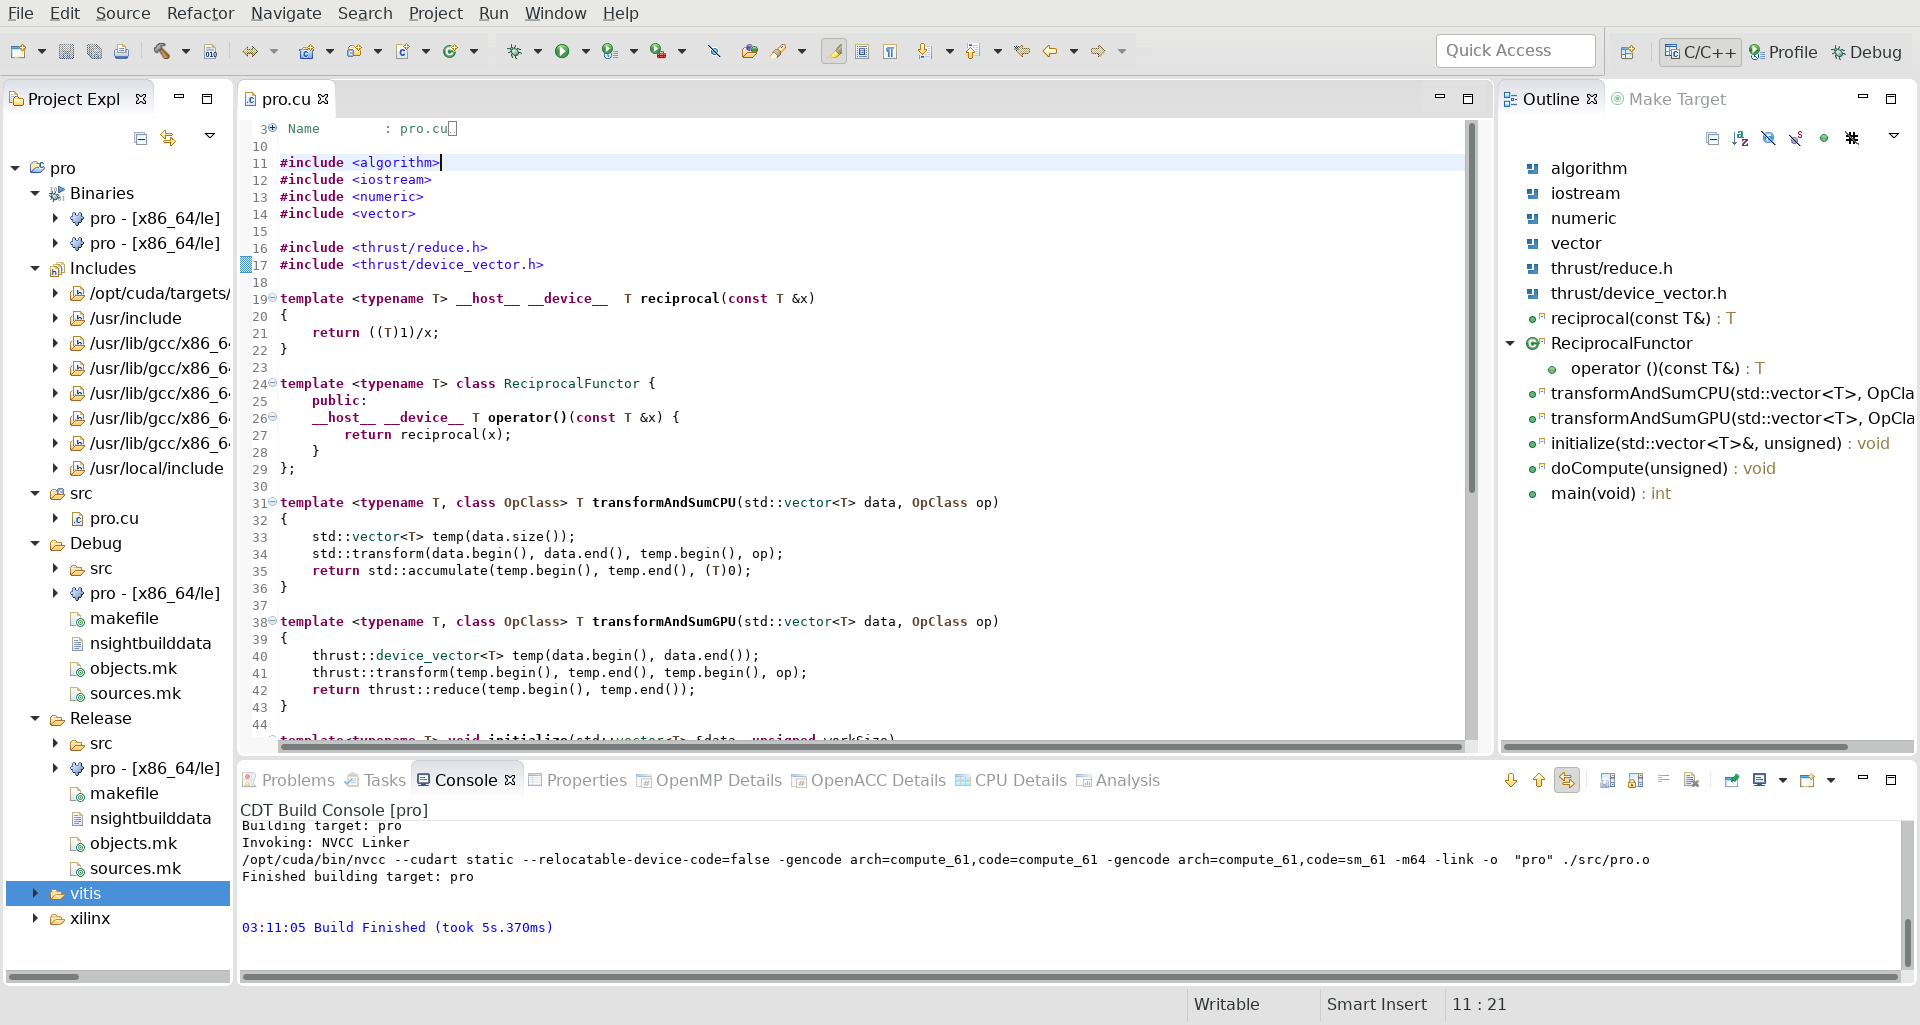
\includegraphics[width=\textwidth]{chapter3/pictures/NEplugin.png}
			            \caption{Nvidia Nsight Eclipse Plugin}
			            \label{fig3:neplugin}
                    \end{figure}
                    \begin{figure}[h]
			            \centering
			            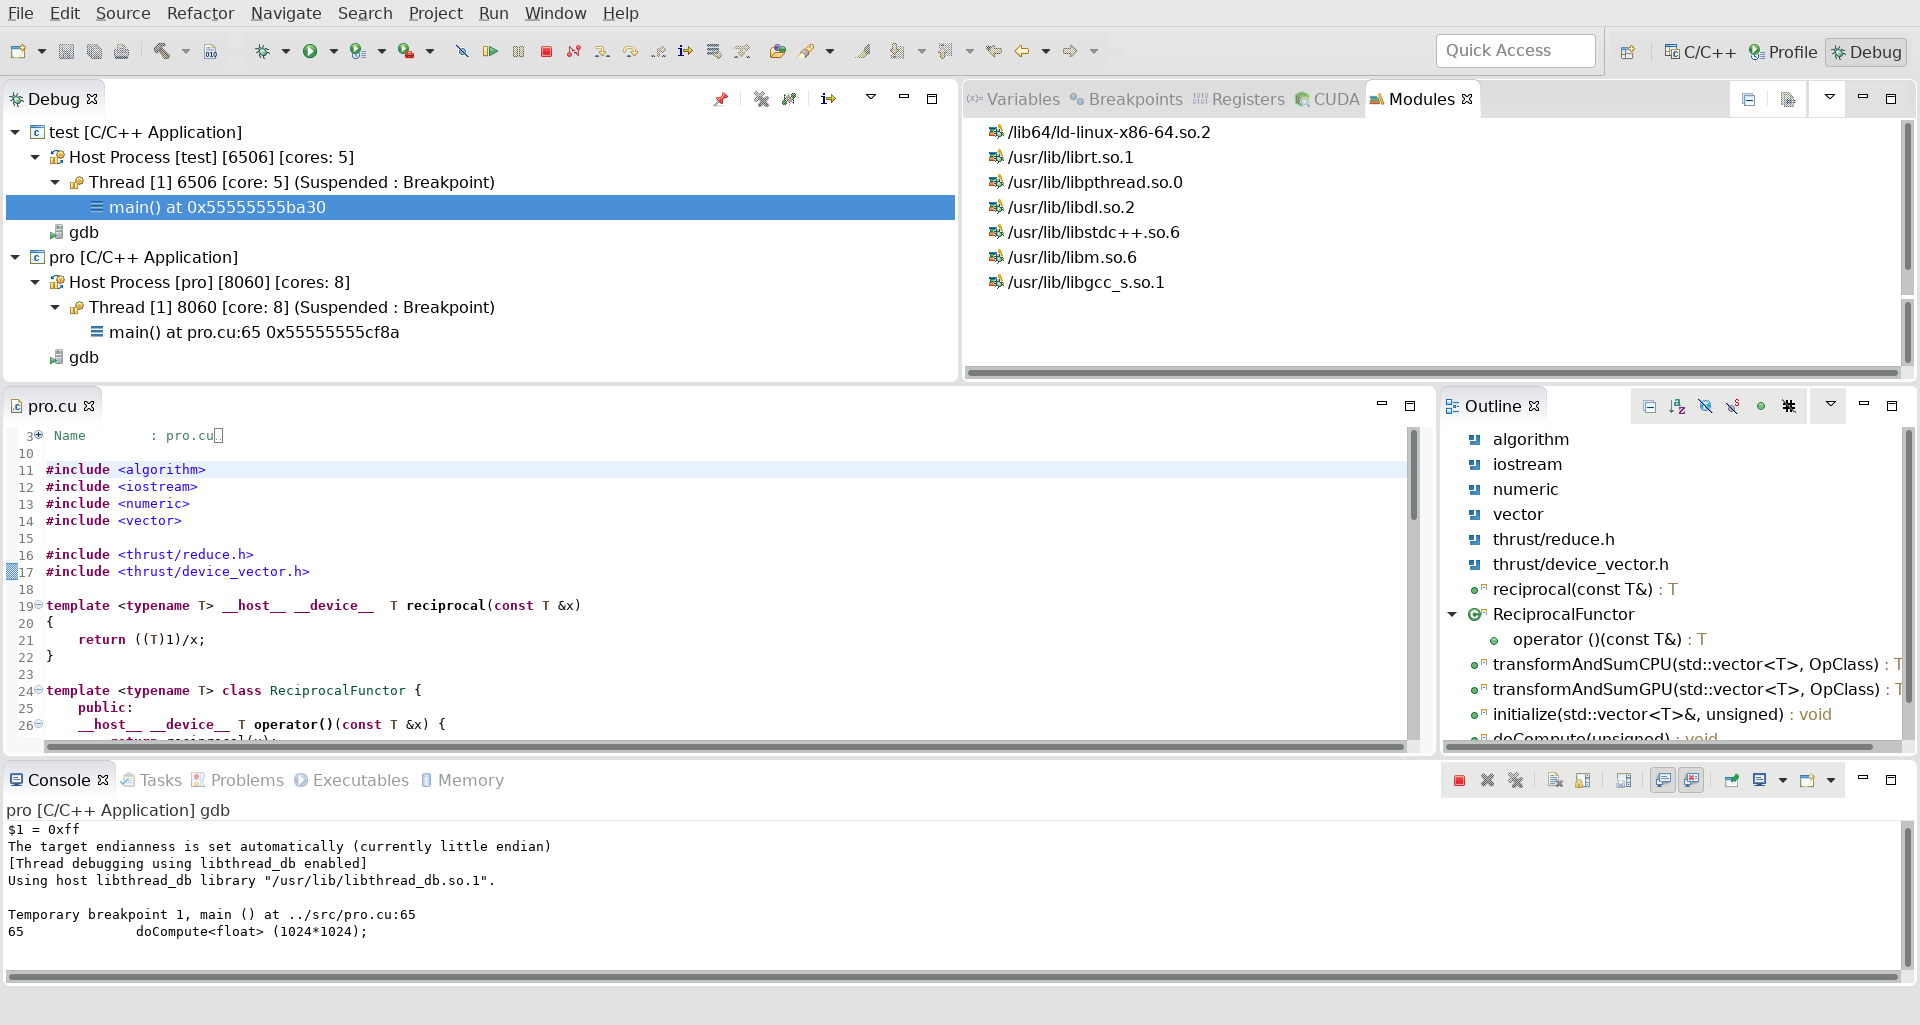
\includegraphics[width=\textwidth]{chapter3/pictures/NEdebug.png}
			            \caption{Nvidia Nsight Eclipse Debugger}
			            \label{fig3:nedebug}
                    \end{figure}
                    \begin{figure}[h]
			            \centering
			            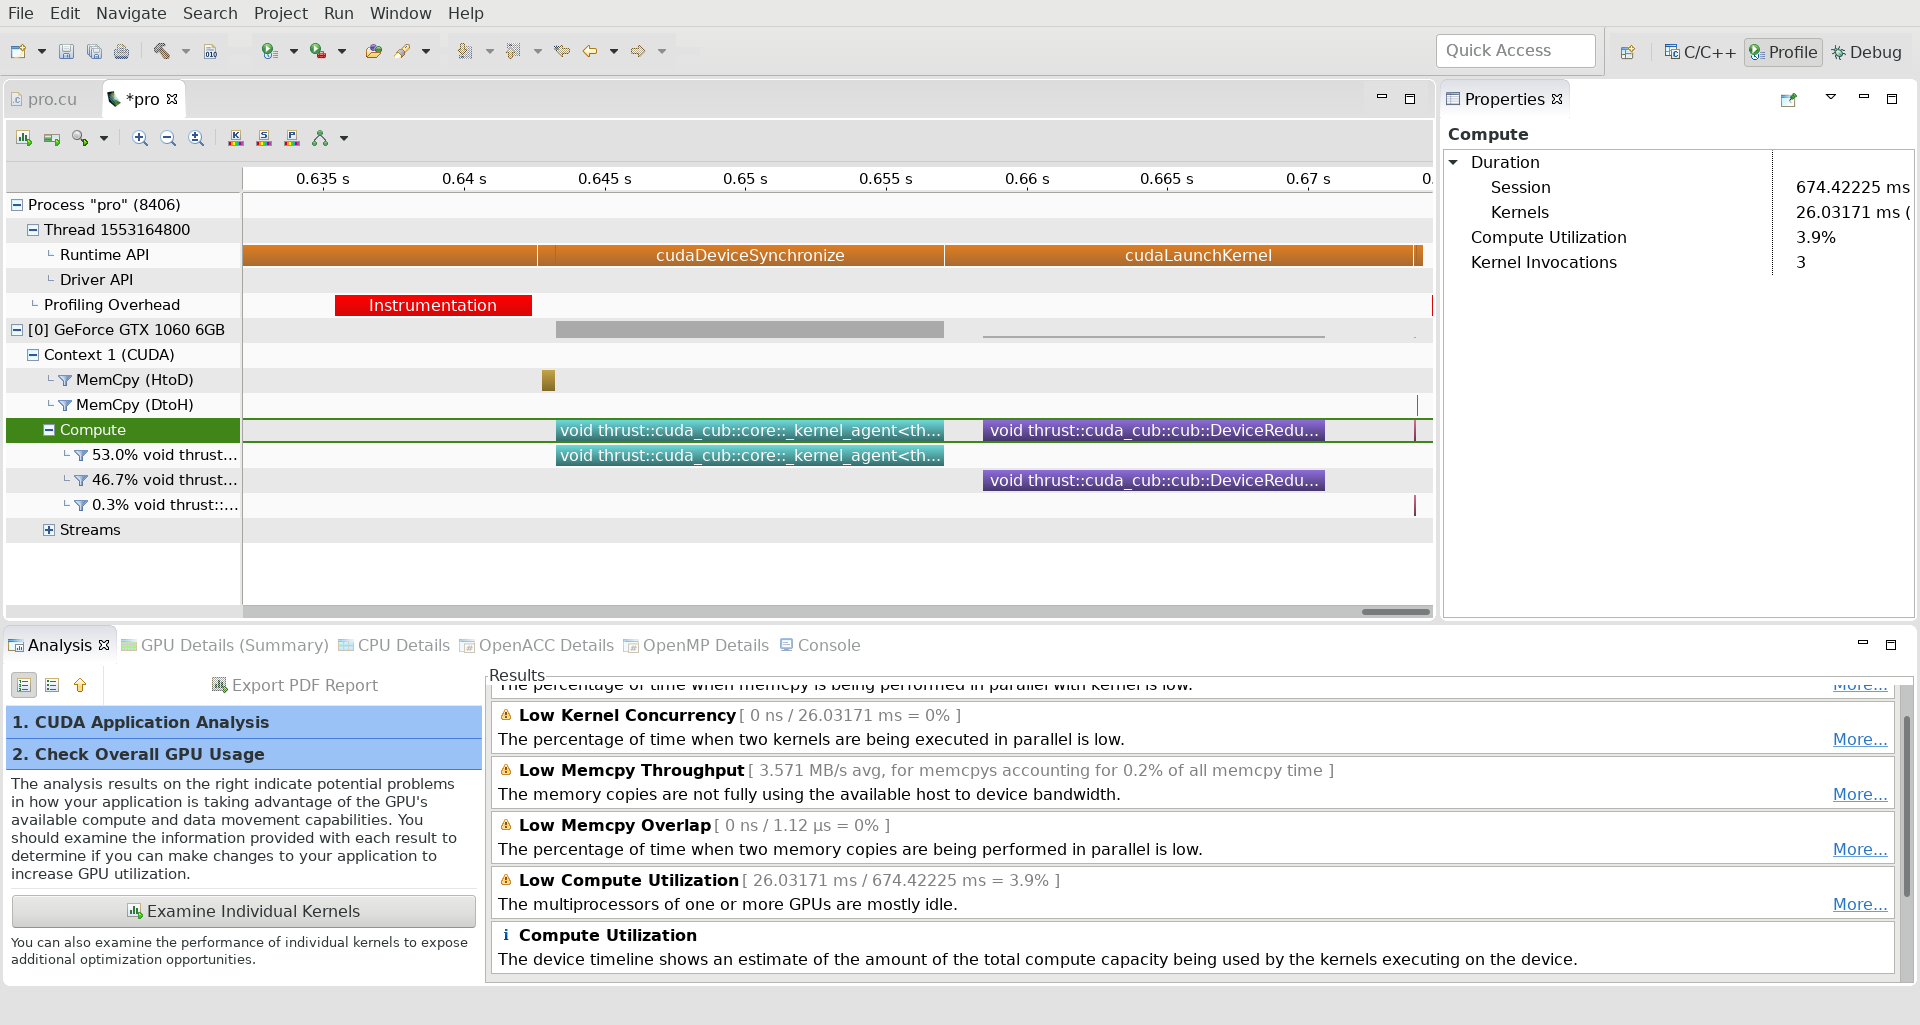
\includegraphics[width=\textwidth]{chapter3/pictures/NEact.png}
			            \caption{Nvidia Nsight Eclipse Performance Analyse}
			            \label{fig3:neact}
			        \end{figure}
			        \FloatBarrier
			    \subsubsection*{Visual Studio Extension}
                    \begin{figure}[h]
			            \centering
			            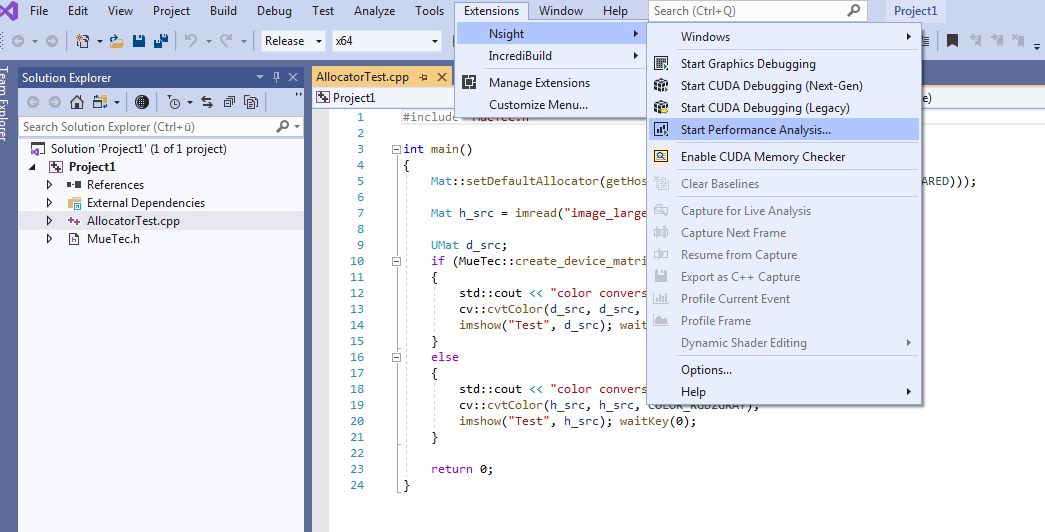
\includegraphics[width=\textwidth]{chapter3/pictures/VSplugin.png}
			            \caption{Nvidia Visual Studio Plugin}
			            \label{fig3:vsplugin}
                    \end{figure}
                    \begin{figure}[h]
			            \centering
			            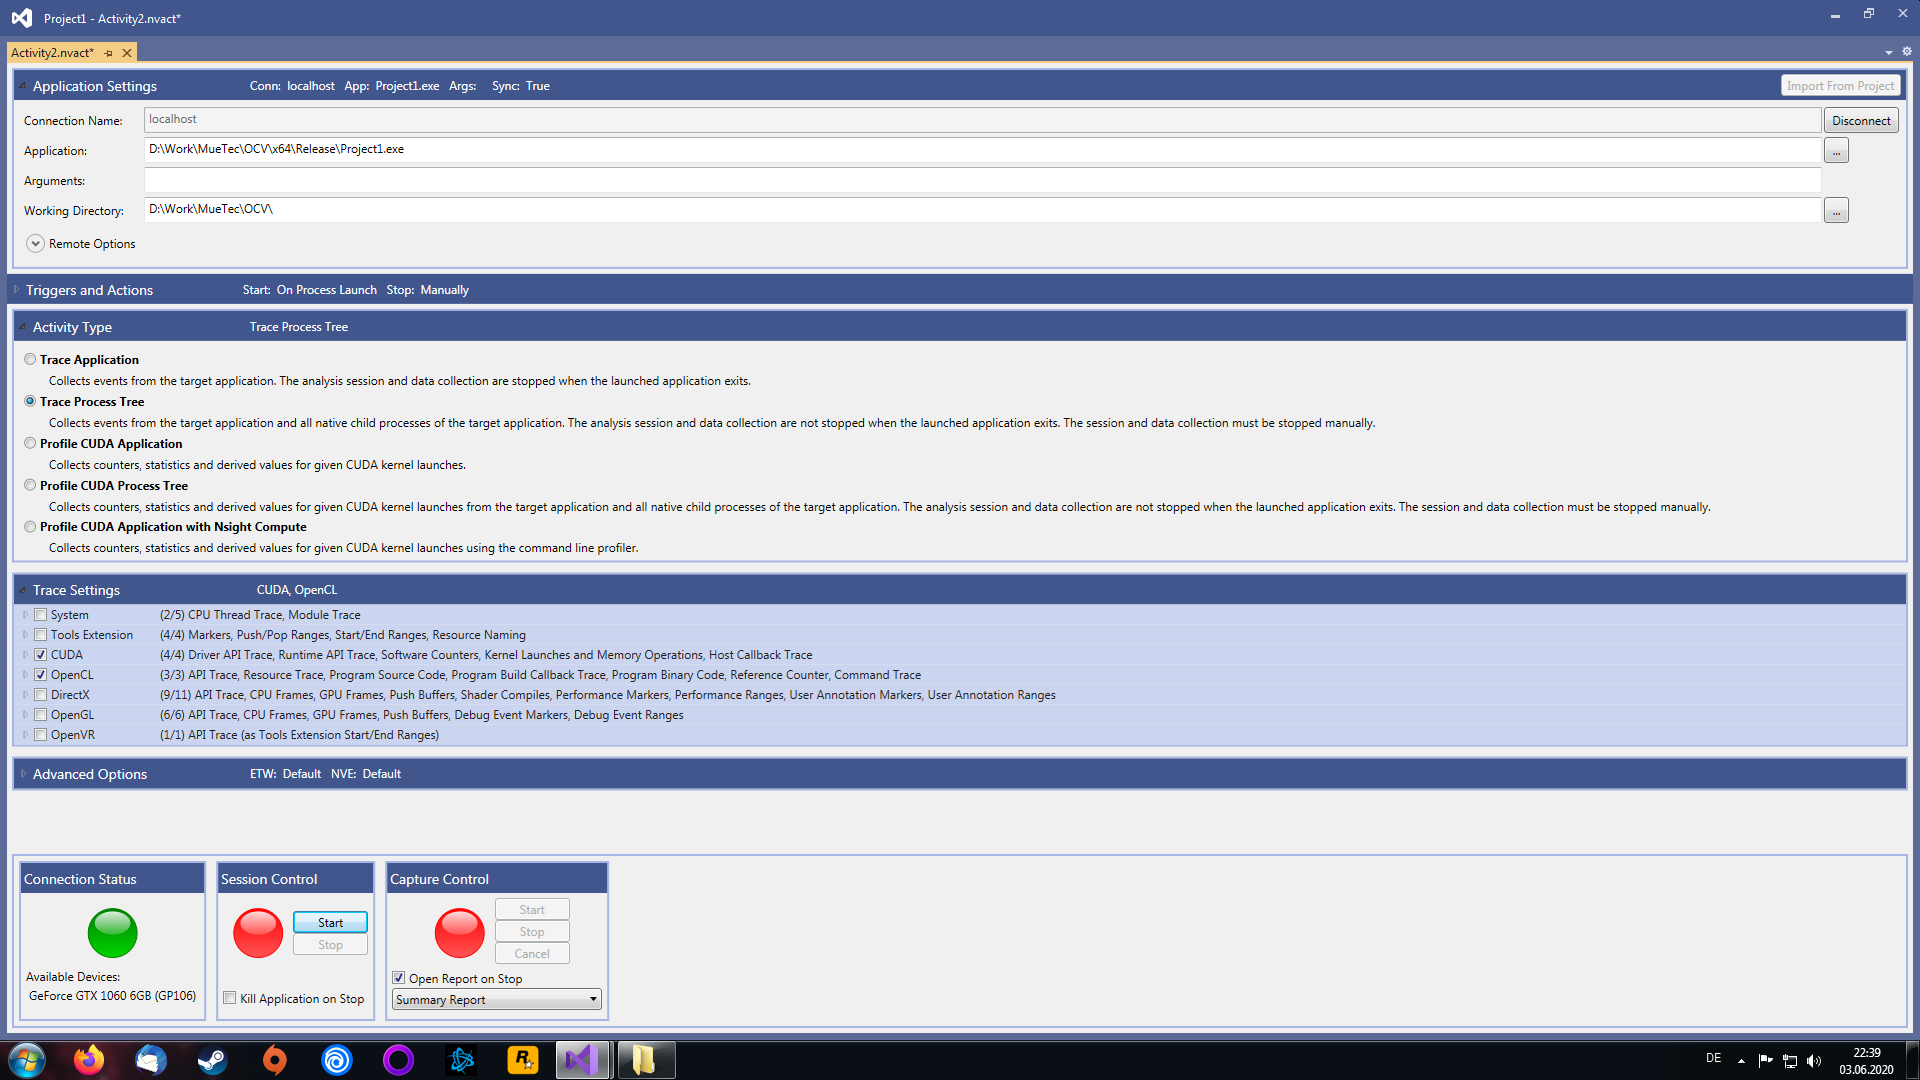
\includegraphics[width=\textwidth]{chapter3/pictures/VSact.png}
			            \caption{Visual Studio Performance Analyse}
			            \label{fig3:vsact}
                    \end{figure}
                    \begin{figure}[h]
			            \centering
			            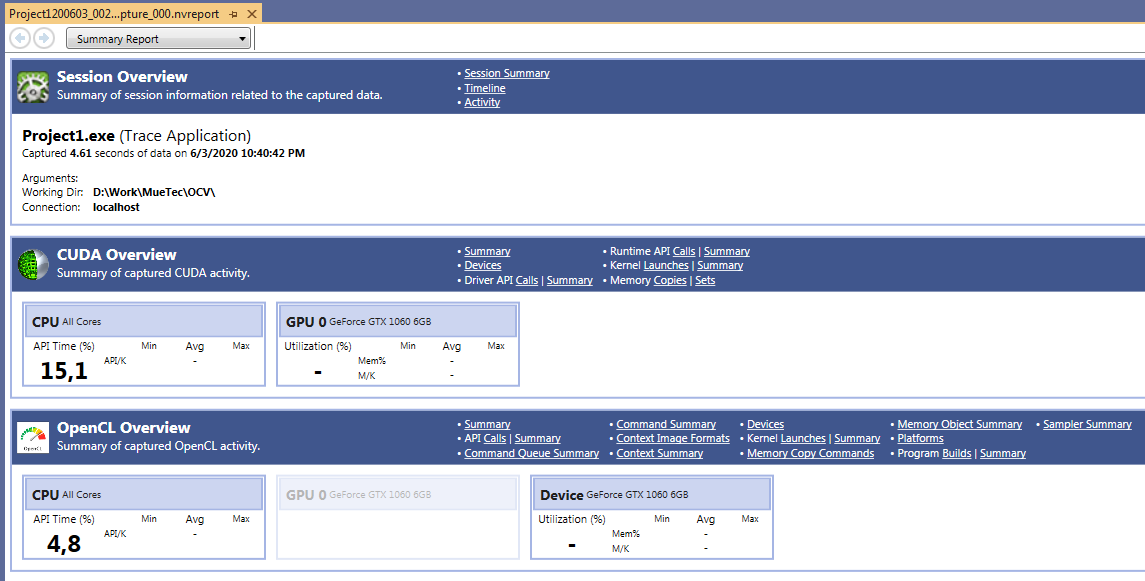
\includegraphics[width=\textwidth]{chapter3/pictures/VSover.png}
			            \caption{Visual Studio Performance Report}
			            \label{fig3:vsover}
                    \end{figure}
                    \begin{figure}[h]
			            \centering
			            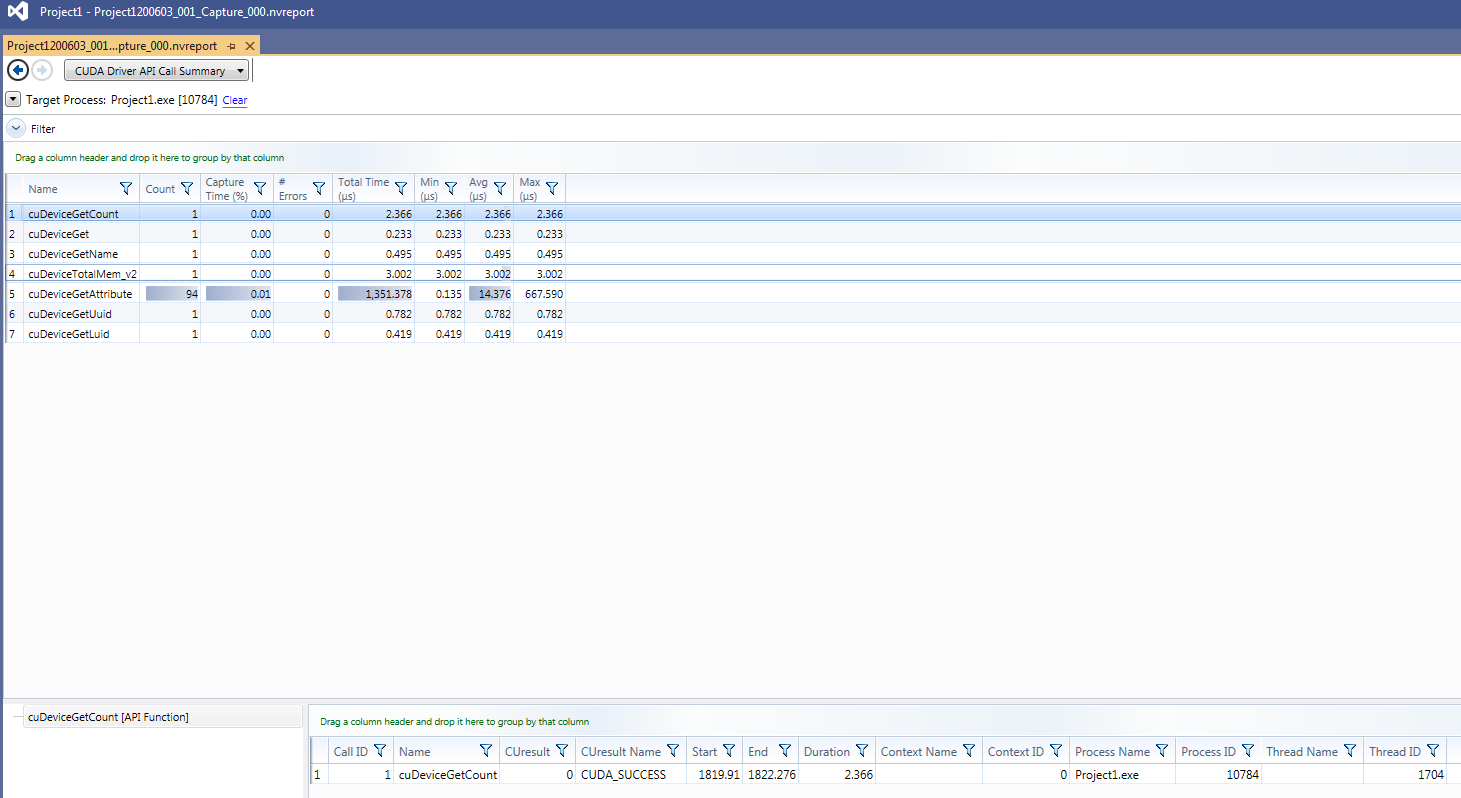
\includegraphics[width=\textwidth]{chapter3/pictures/VSapi.png}
			            \caption{Visual Studio API Calls}
			            \label{fig3:vsapi}
			        \end{figure}
			        \FloatBarrier
			\subsection{nvprune}
			\subsection{nvdisasm und cuobjdump}
		
